\section{Rolling Stock Management}

The Rollingstock view provides a complete inventory of all rolling stock registered in the system. Selecting "Rollingstock" from the navigation drawer displays the main tabular view containing all registered pieces, including key attributes such as Road Name, Road Number, AAR Code, Description, Color, and available Action buttons. Figure \ref{fig:rollingstock} displays the main Rollingstock table page.

\begin{figure}[H]
    \centering
    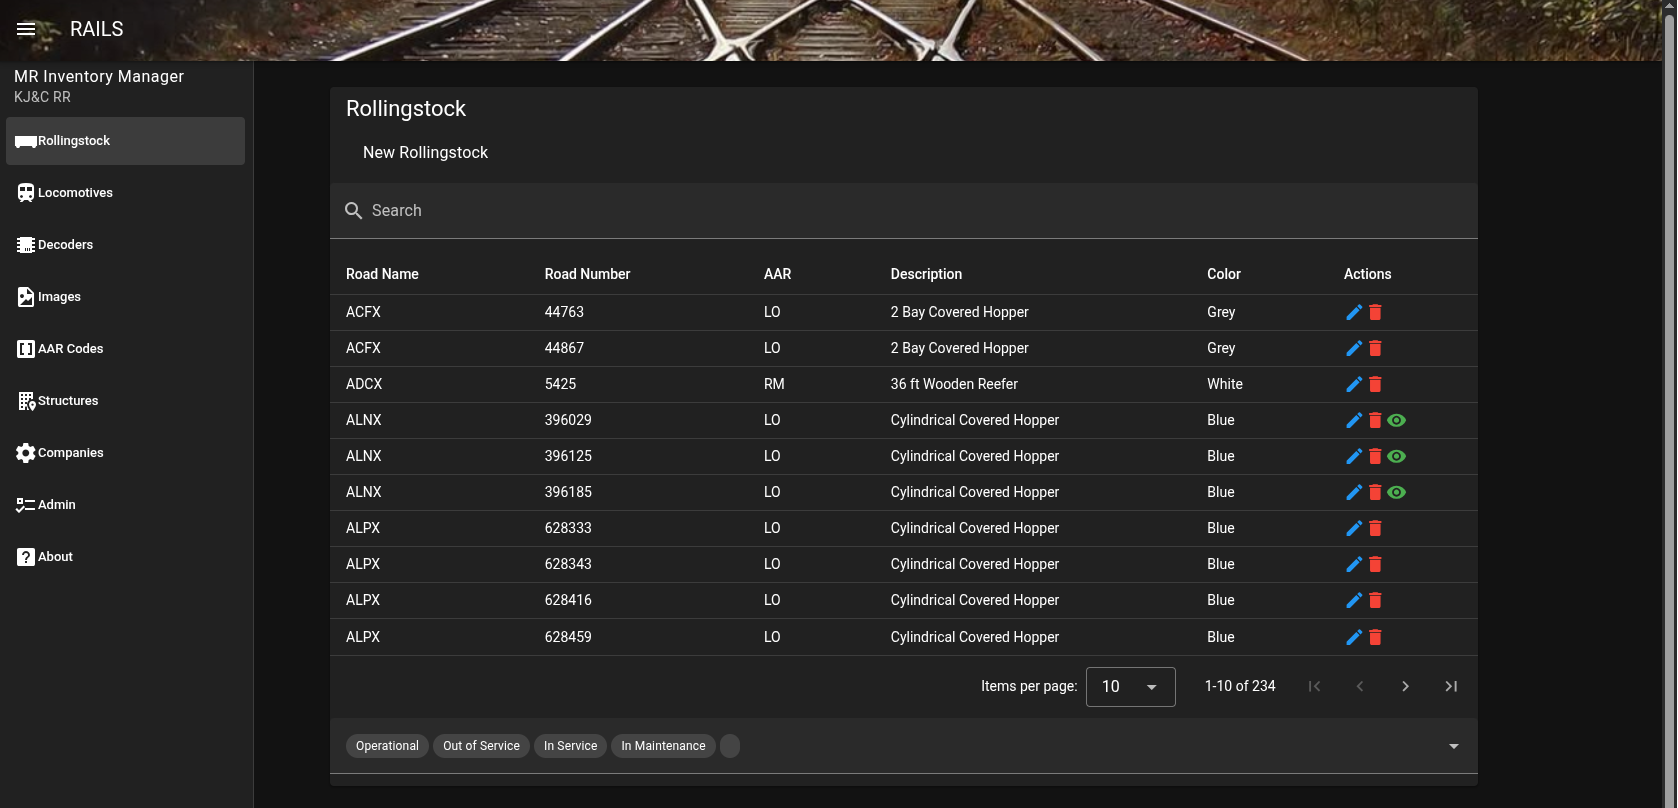
\includegraphics[width=0.85\textwidth]{./images/rollingstock.png}
    \caption{Rollingstock Page}
    \label{fig:rollingstock}
\end{figure}

\subsection{Page Quantity Selection}

The table displays items in paginated format. Users can control the number of rolling stock items shown per page using the dropdown selector located at the bottom right of the table. Available options include 10, 25, 50, 100, or All items. Figure \ref{fig:rs-pg-qty} illustrates changing the items per page display count.

\begin{figure}[H]
    \centering
    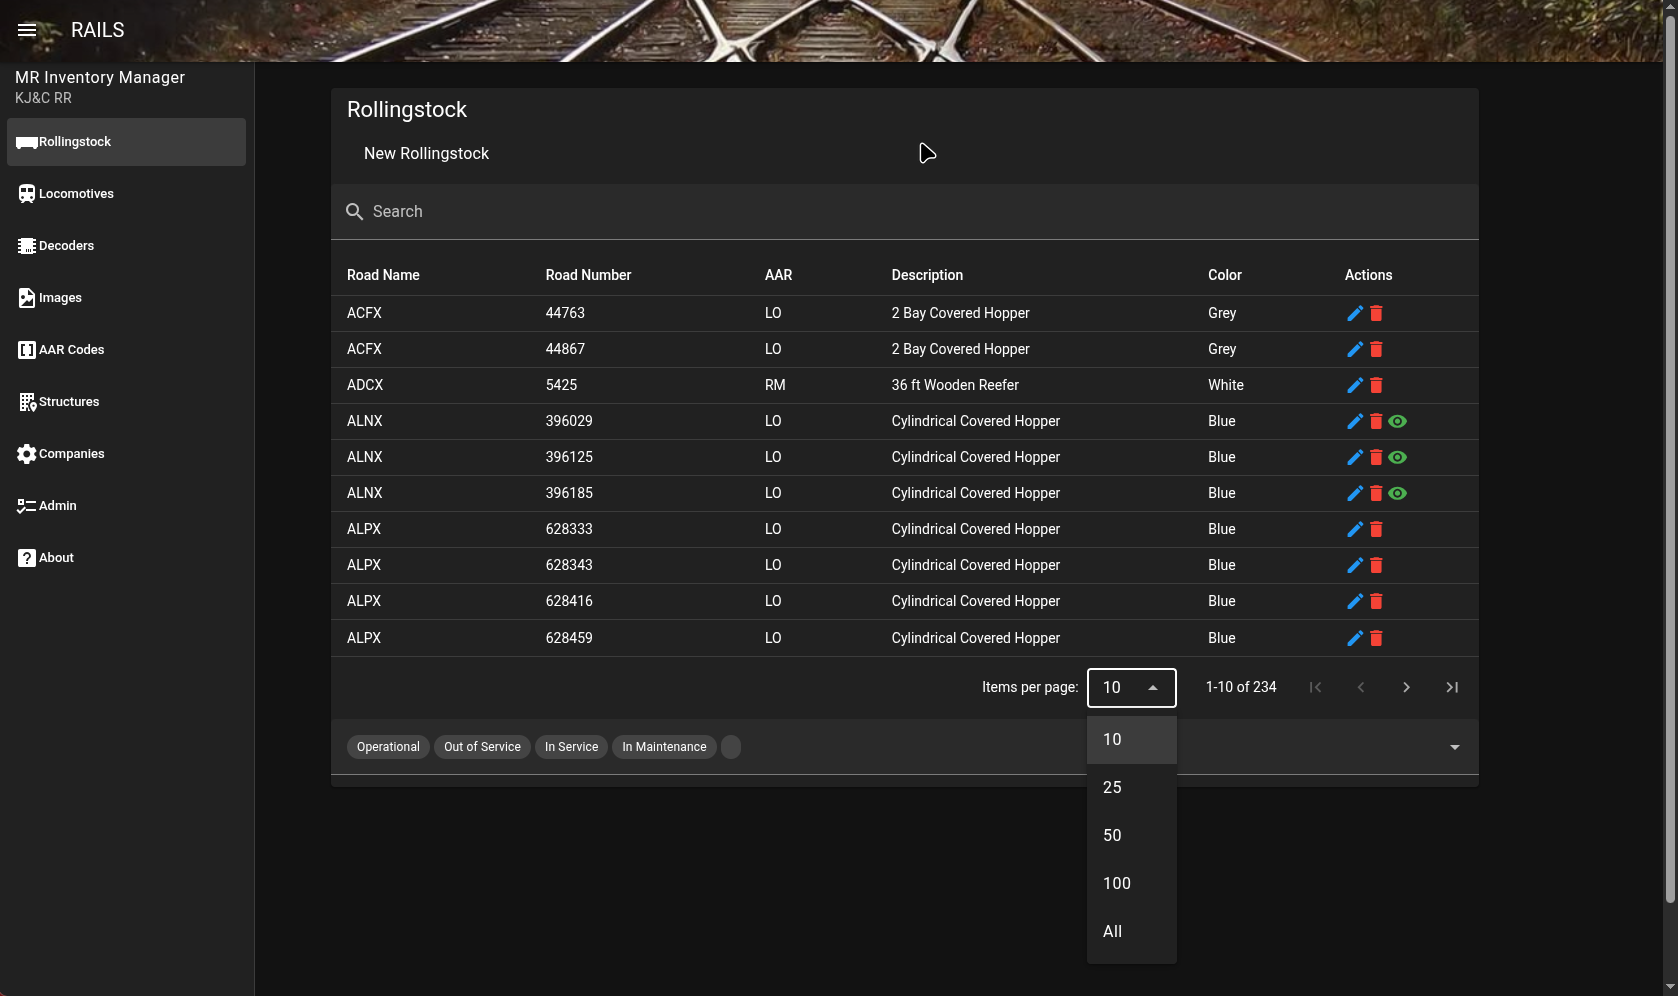
\includegraphics[width=0.85\textwidth]{./images/rs-pg-qty.png}
    \caption{Items Per Page Selection}
    \label{fig:rs-pg-qty}
\end{figure}

\subsection{Status Filtering}

Rolling stock entries can be filtered dynamically based on operational status. At the bottom of the view, status filter controls allow toggling visibility for items designated as Operational, Out of Service, In Service, or In Maintenance. Figure \ref{fig:rs-status} shows the operational status filtering interface open.

\begin{figure}[H]
    \centering
    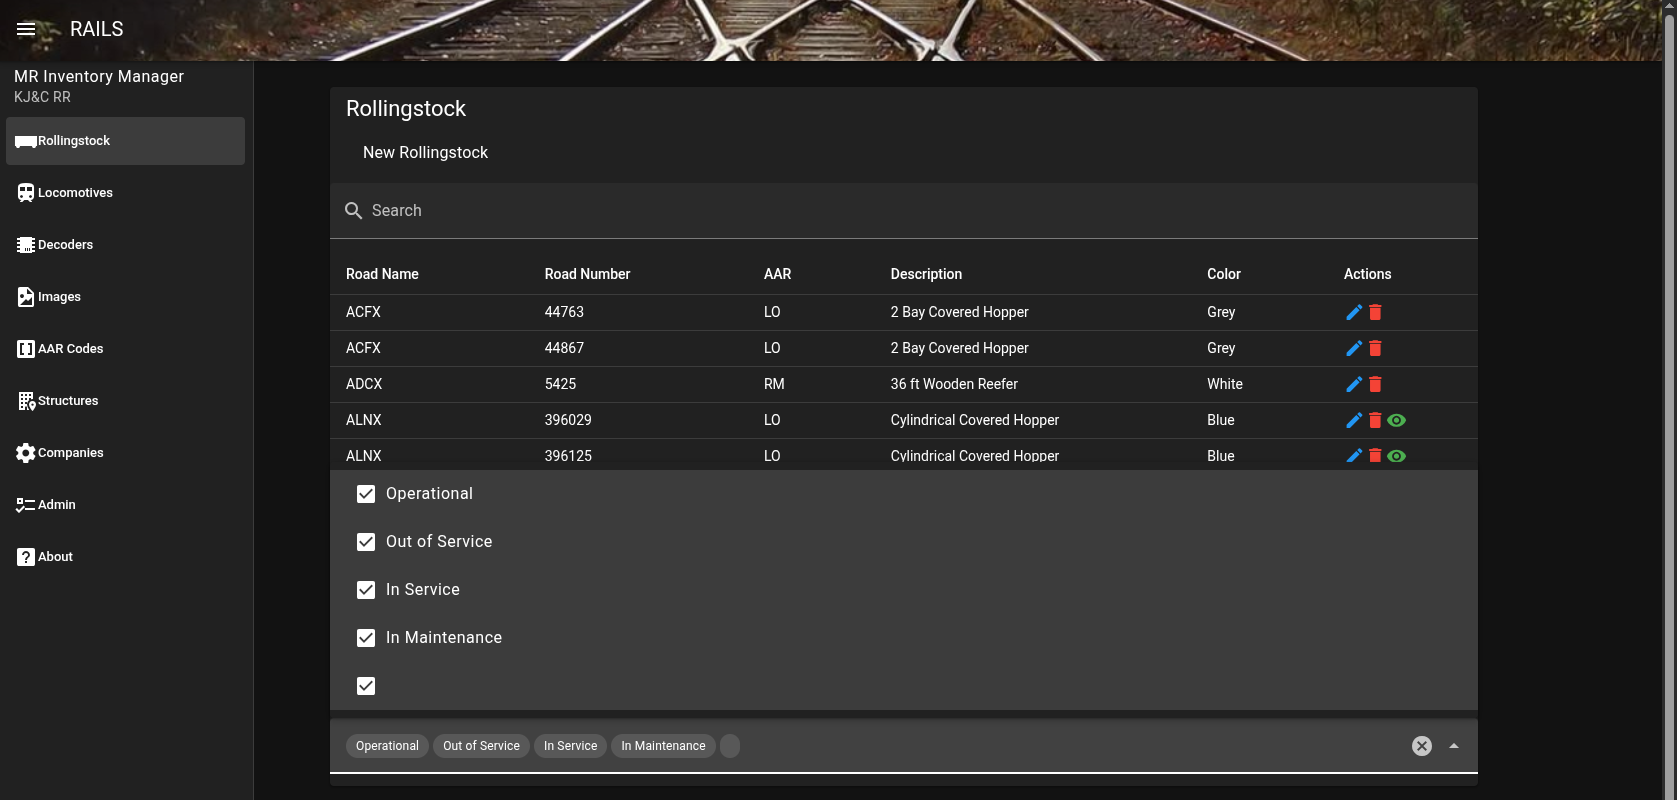
\includegraphics[width=0.85\textwidth]{./images/rs-status.png}
    \caption{Status Filter}
    \label{fig:rs-status}
\end{figure}

\subsection{Search Functionality}

A search bar located above the main table enables real-time filtering across rolling stock attributes. Typing search terms such as a road name (e.g., "cnw") instantly filters the list to show matching records. Figure \ref{fig:rs-search} shows filtered search results.

\begin{figure}[H]
    \centering
    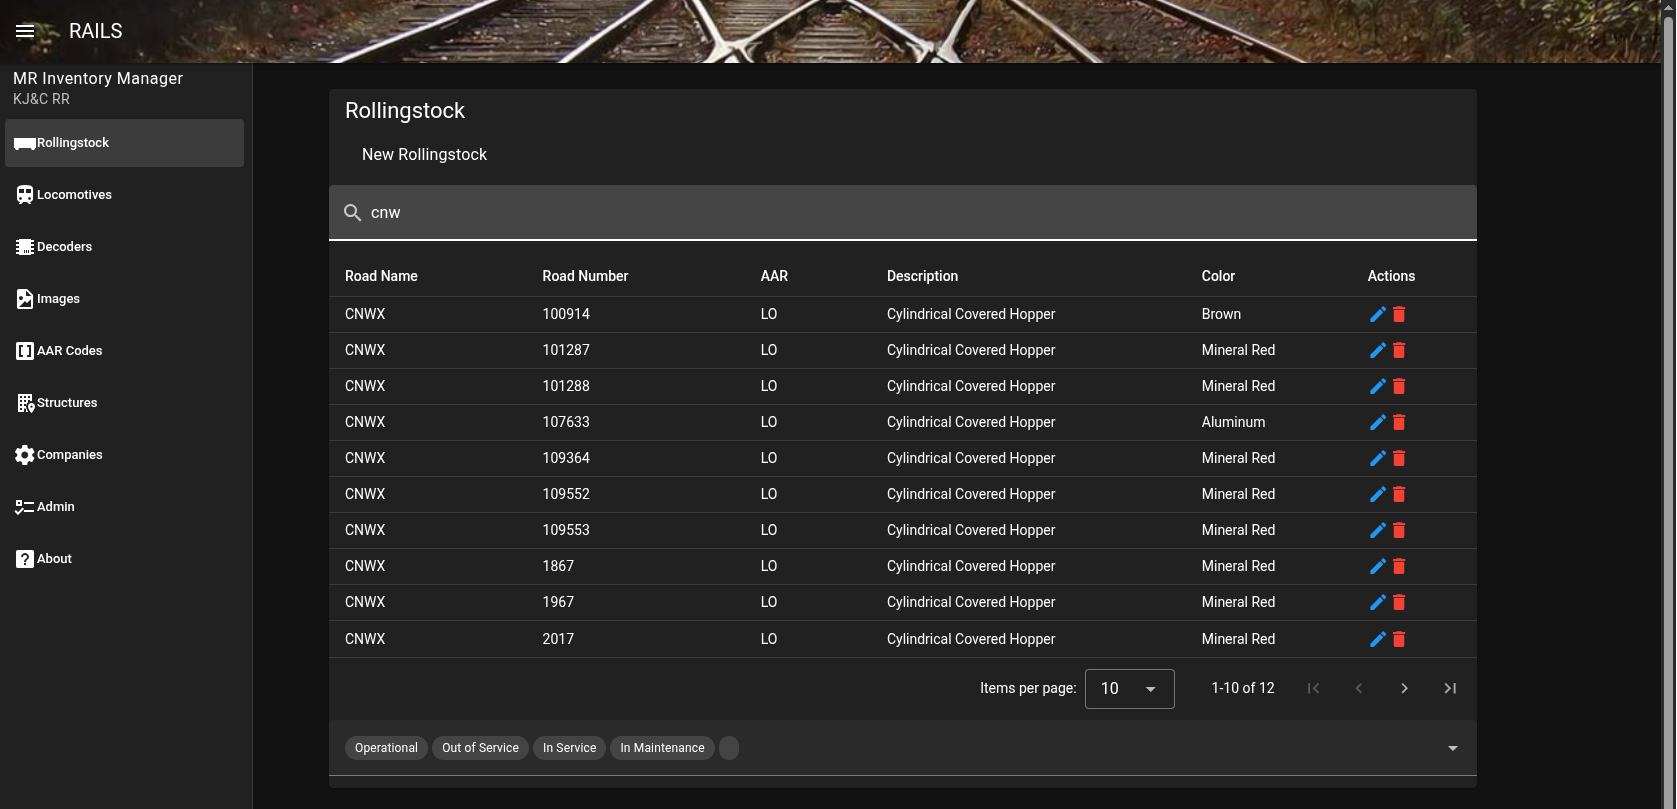
\includegraphics[width=0.85\textwidth]{./images/rs-search.png}
    \caption{Search Rollingstock}
    \label{fig:rs-search}
\end{figure}

\subsection{Viewing Rollingstock Details}

For entries configured with associated image files, an eye icon appears under the Actions column. Clicking this icon opens the Rollingstock Details dialog, displaying comprehensive prototype specifications, dimensions, status, and a photograph of the equipment. Figure \ref{fig:rs-view} shows the detailed view modal for a selected car.

\begin{figure}[H]
    \centering
    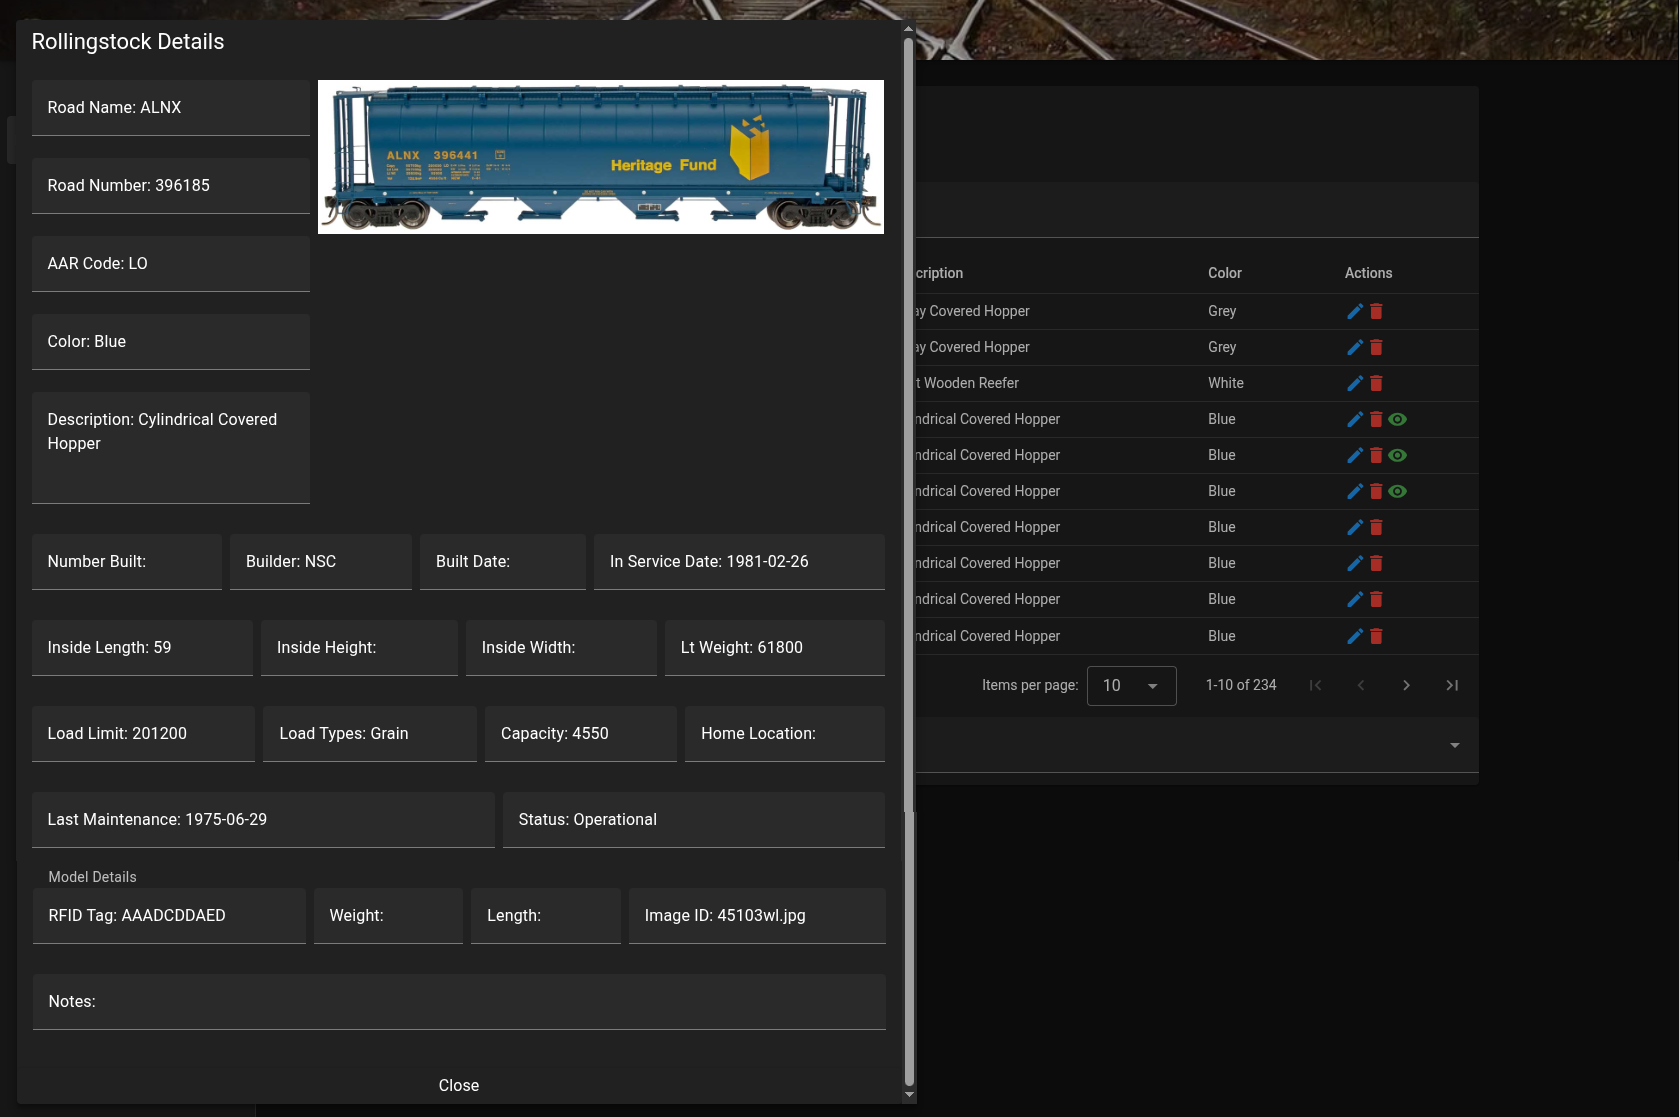
\includegraphics[width=0.85\textwidth]{./images/rs-view.png}
    \caption{View Rollingstock Details}
    \label{fig:rs-view}
\end{figure}

\subsection{Adding New Rollingstock}

Clicking the "New Rollingstock" button above the table opens a blank data entry form. Users can populate fields including road information, dimensions, load characteristics, model parameters, RFID tag associations, and linked image IDs. Figure \ref{fig:rs-new} shows the entry form for creating a new rolling stock item.

\begin{figure}[H]
    \centering
    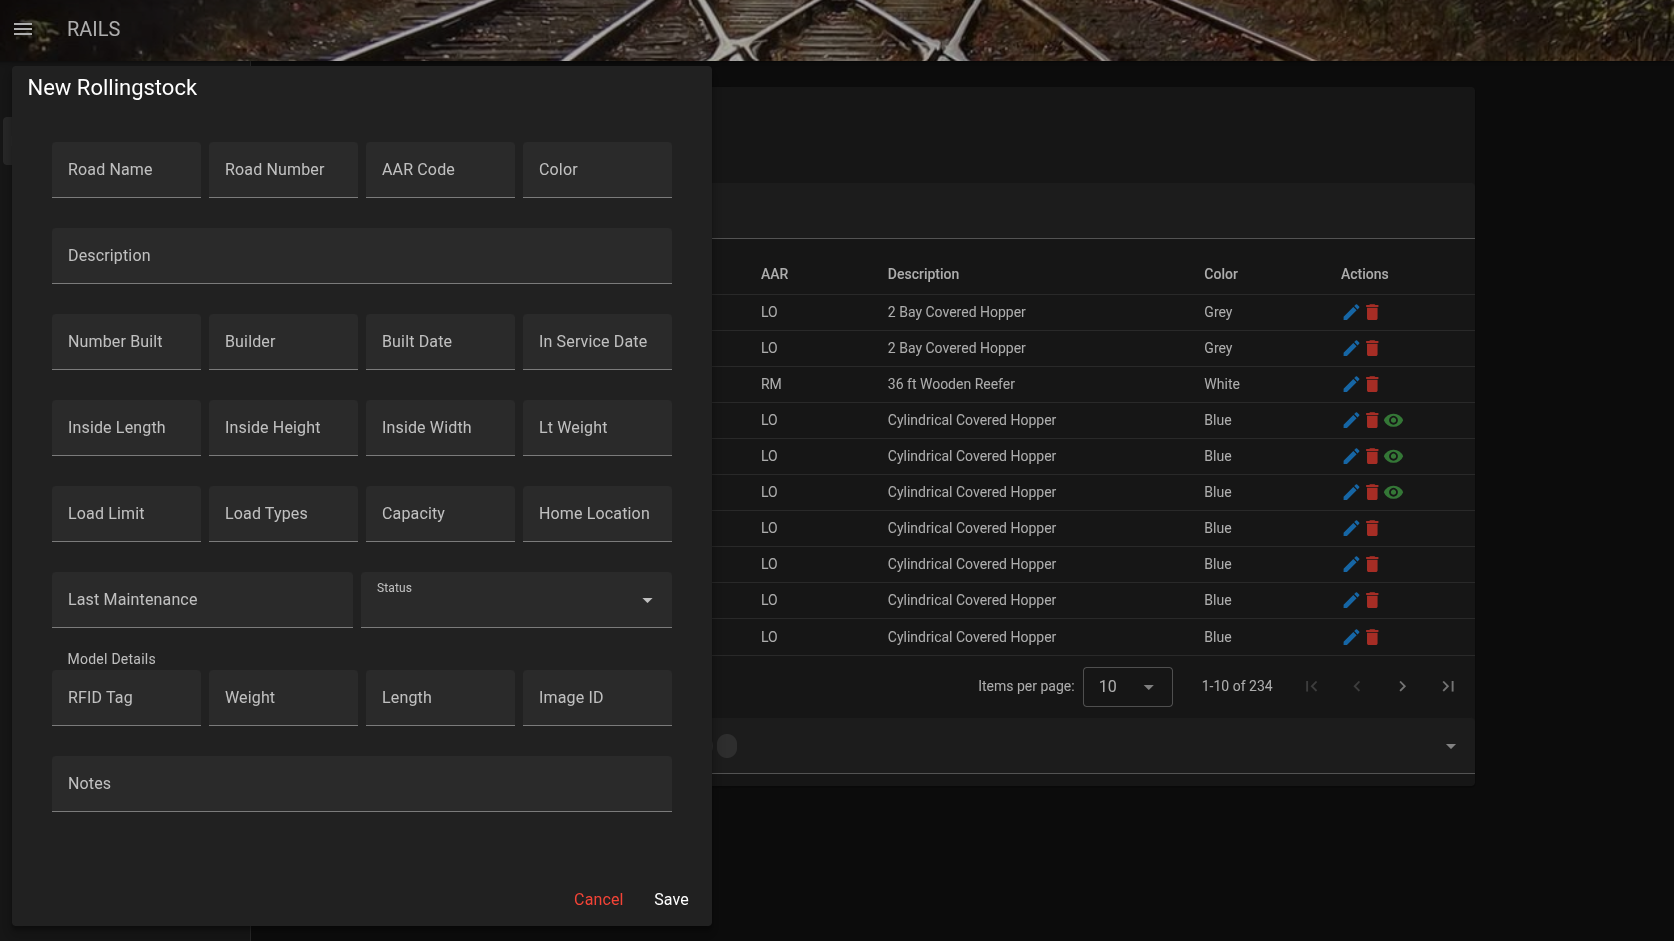
\includegraphics[width=0.85\textwidth]{./images/rs-new.png}
    \caption{New Rollingstock Entry}
    \label{fig:rs-new}
\end{figure}

\subsection{Editing Rollingstock Records}

To modify an existing entry, click the blue pencil icon in the Actions column for that row. This opens the details dialog in editable mode, populated with current record data for updating field values. Figure \ref{fig:rs-edit} illustrates editing an existing record.

\begin{figure}[H]
    \centering
    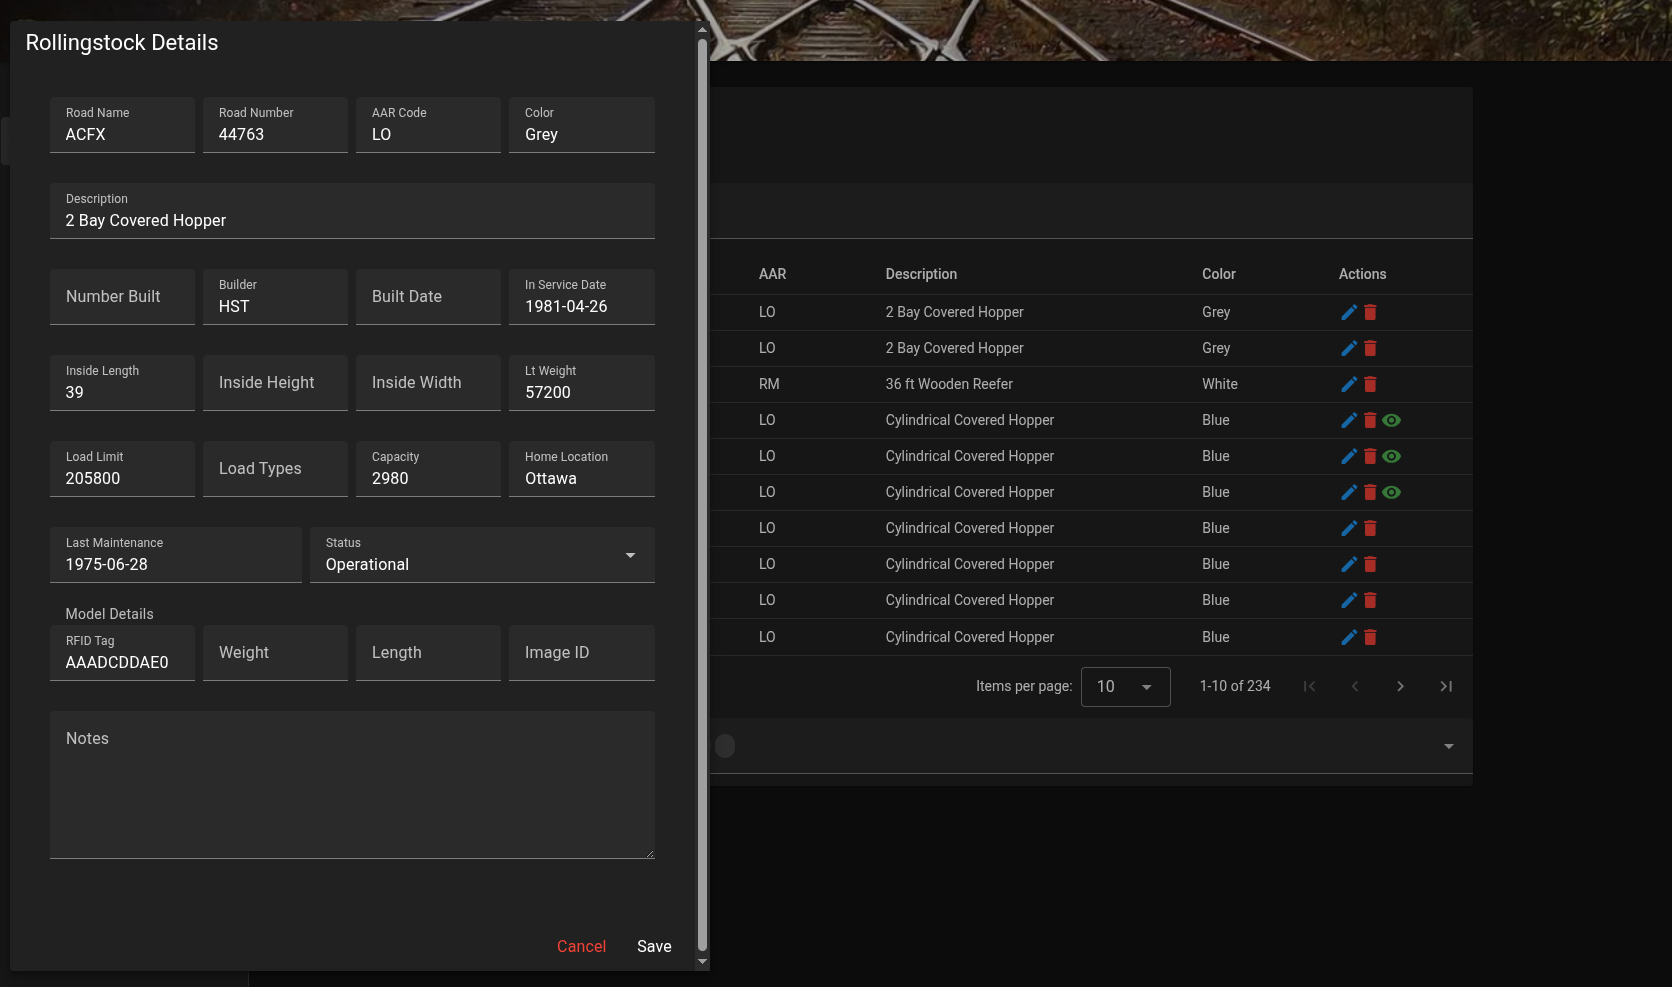
\includegraphics[width=0.85\textwidth]{./images/rs-edit.png}
    \caption{Edit Rollingstock}
    \label{fig:rs-edit}
\end{figure}

\subsection{Deleting Rollingstock Records}

To remove a record from the database, click the red trash bin icon in the Actions column. A confirmation dialog appears requesting confirmation before permanently removing the record. Figure \ref{fig:rs-delete} shows the deletion confirmation prompt.

\begin{figure}[H]
    \centering
    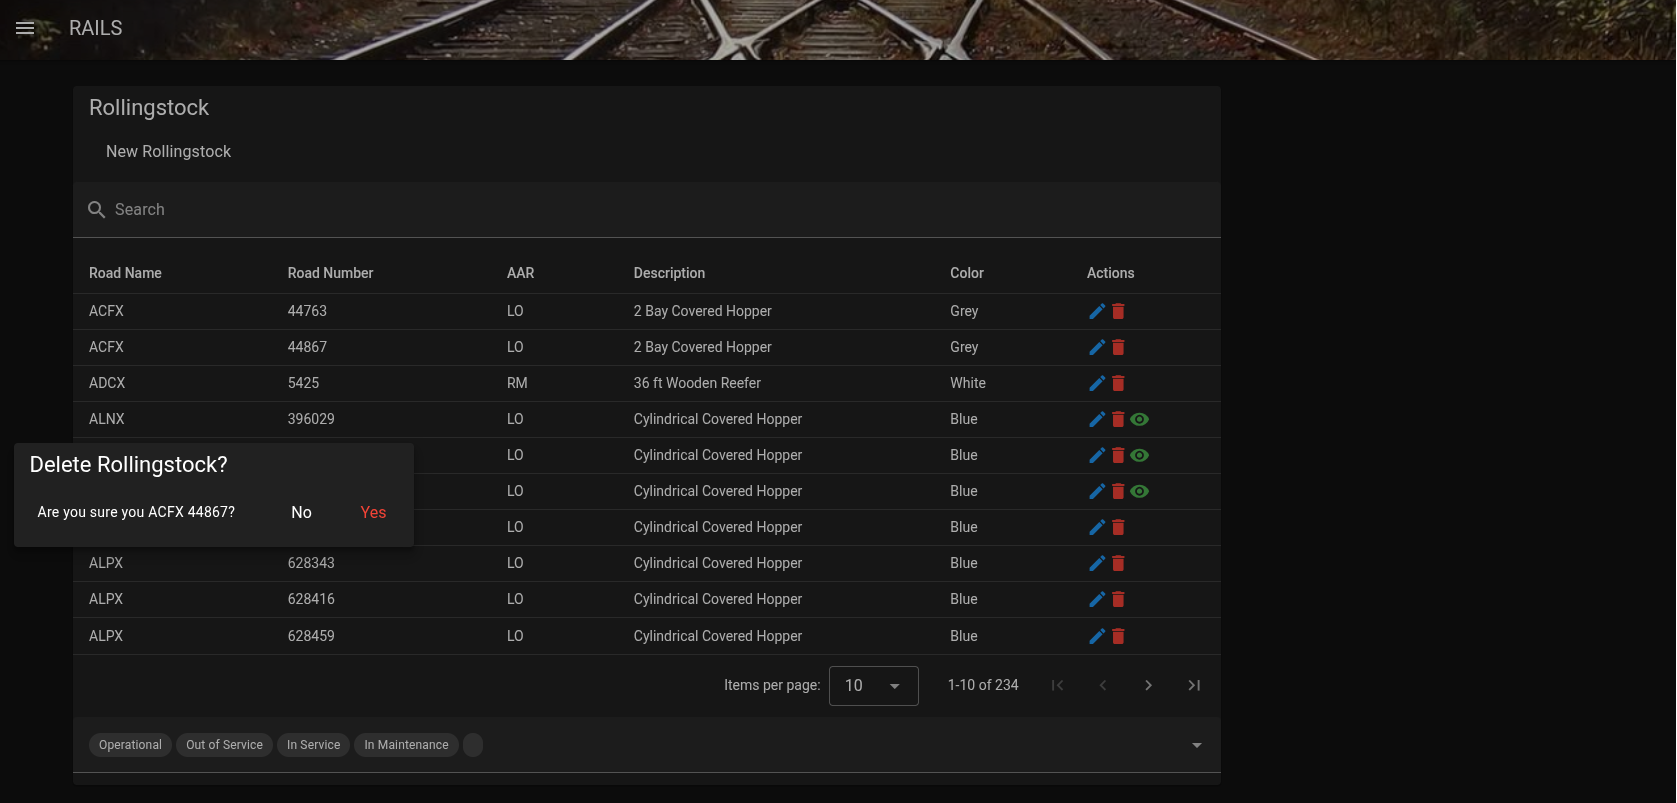
\includegraphics[width=0.85\textwidth]{./images/rs-delete.png}
    \caption{Delete Rollingstock Confirmation}
    \label{fig:rs-delete}
\end{figure}
